\documentclass{article}
\author{Jonathan Dyer}
\title{CS 1699: Privacy in the Electronic Society \\
        \textit{Project 2 -- Access Control Policies}}

\usepackage{amsmath}
\usepackage{amsthm}
\usepackage{enumitem}
\usepackage[margin=0.8in]{geometry}
\usepackage{graphicx}
\usepackage[backend=bibtex,type=alphabetical,sorting=ynt]{biblatex}
\addbibresource{p2.bib}

% ============ USED FOR MY FORMAT ============
\providecommand{\task}[1]{\section{Task #1}}
\providecommand{\soln}{\textbf{Solution: }}
\providecommand{\image}[1]{
    \begin{center}
        \includegraphics[width=1.0\textwidth]
            {#1}
    \end{center}
}
\providecommand{\tightlist}{
    \setlength{\itemsep}{0pt}\setlength{\parskip}{0pt}
}
\providecommand{\inlinecode}{\texttt}
\providecommand{\RT}{\textbf{RT}}

% ============ USED FOR CODE LISTINGS ============
\usepackage{listings}
\usepackage[usenames,dvipsnames,svgnames]{xcolor}
\definecolor{javagreen}{rgb}{0.25,0.5,0.35}
\lstset{
    basicstyle          = \footnotesize,
    commentstyle        = \color{javagreen},
    frame               = single,
    language            = XML,
    stringstyle         = \color{orange},
    numbers             = left,
    showstringspaces    = false,
    deletekeywords      = {len, max, format, min},
    morekeywords        = {yield, function, then, do, to},
    keywordstyle        = \color{blue},
    mathescape
}

\setcounter{secnumdepth}{0} % sections are level 1


\begin{document}
\maketitle

\tableofcontents

\task{W0}
\subsection{$\RT_0$: Role-based Trust management with attributes}
The access-control language selected for this project is a simplified variant of a family of expressive languages known as $\RT$, which is short for \textit{\textbf{R}ole-based \textbf{T}rust-management}.
In spite of the name, the $\RT$ family is actually an extension of role-based access control (RBAC) known as \textit{attribute}-based access control (ABAC).
It fulfills all of the desirable traits mentioned in \cite{RTmain}, including delegation of attribute authority, inference of attributes, and more.
By allowing explicit subject abstraction and specific attribute assignment to those subjects, the system provides the same functionality that roles do via selection by attributes and intersection of attributes along with even greater flexibility and expressiveness.
The language utilized here is based on a combination of $\RT_0$ and $\RT_2$, and functions as follows: \\
\begin{itemize}
  \item The primary structures in this framework are \textit{entities} (or principals), \textit{subjects} (or users), \textit{roles} (which contain rights or permissions), and \textit{objects} (or resources).
  \item \textbf{Entities} are simply the organizations or systems that issue credentials (i.e. assign roles to users). By explicitly abstracting entities, the $\RT$ framework allows for localized roles, as well as more extensive delegation.
  \item \textbf{Subjects} are the users or agents in the system. They may have one or more roles that provide them with permissions (or authorized actions) for accessing objects in the specified way.
  \item \textbf{Roles} are a convenient way of grouping permissions that may be assigned to subjects. Roles may be hierarchical--if a role dominates another, then it has every permission the other role has. This helps reduce the number of roles and relationships that have to be dealt with in the system. Role assignment may be achieved by specifying subject attributes.
  \item \textbf{Objects} are the elements whose access is being controlled by this entire schema. They may be grouped by attribute as well, allowing flexible and powerful specification of permissions.
  \item Each structure accepts descriptive \textit{attributes} that enable powerful specification of policies based on any desired combination of subject, role, or object attributes. This, in conjunction with the outline above, facilitates the following features (among others): \\
  \begin{enumerate}
    \item \textbf{Indirection}: Because we can specify policies according to attributes, we may assign i) a set of permissions (i.e. a role or multiple roles), to ii) a set of users, over iii) a set of objects, as long as those sets can be well-defined or uniquely specified (i.e. all elements in the desired set must share an attribute that specifies exactly that set).
    \item \textbf{Delegation}: Different entities that assign roles (within their domain) may easily defer to the authority of another entity for checking role membership. That is to say, if organization $A$ defines role $r_1$, it is simple to write a policy that includes into $r_1$ all members of role $r_2$ from some other organization $B$ as well. This is also referred to as 'delegation of attribute authority', meaning that if $B$ says that some subject has attribute $r_2$, then $A$ says it has attribute $r_1$ (here speaking of roles as attributes of users). Details of how this is done are given in the next section.
    \item \textbf{Role Hierarchy}: Roles may inherit permissions from other roles given by the same entity. This is a variant of delegation, in a sense allowing an organization to delegate authority over some role attribute to that same organization under another role attribute. Thus, role management is simplified and duplication is reduced.
    \item \textbf{Attribute Intersection}: Support of multiple attributes on any given element in the system also allows specification of policies by intersection of attributes. For instance, it is possible to specify an action that is allowed only for users who are in the intersection of multiple roles (i.e. users that have each of those roles).
    \item \textbf{Logical Objects}: Inspired by $\RT_2$, the current variation of this framework also supports collections of objects, known as Object Groups, which allows addition by attribute and assignment of permissions respecting objects \textit{en masse}. In other words, it is possible to define a role with an access mode and an entire group of logically-related objects (via attributes) rather than just one object at a time.
  \end{enumerate}
\end{itemize}
It is important to note that there are many other extensions and variations in the $\RT$ language family, and the current iteration was chosen as a convenient balance between expressiveness and feasibility for the purposes of the current project. Many other features are possible within the $\RT$ framework, such as parameterization of attributes, threshold policies, and more. \par
Further, it is important to note that the original specification of $\RT$ also included details regarding the issue of \textit{common vocabularies} across entities. This issue of vocabularies or namespaces is dealt with via \textit{application domain specification documents (ADSDs)}, but was ommitted here for brevity's sake, and because it is not relevant to the ideas being explored. For more information however, and generally for a great amount of detail regarding the $\RT$ family of languages, see \cite{RTmain} and \cite{RTold}.


\section{Task W1}
\subsection{Overview of Syntax and Policy File Format}
The syntax chosen to write policy files for the above language is straightforward and designed for maximal ease and clarity. It is encoded in XML, and comprises two primary sections in every entity for which policies are being defined: 1) Data, and 2) Policies. \par
\textbf{Data} is where all elements of the system are specified, and includes the following: \\
\begin{itemize}
  \item A full definition of any objects in the system, including object groups and any attributes associated with them.
  \item A definition of all roles and their corresponding permissions, including all objects/object groups those roles affect and any role hierarchy that exists natively (independent of any particular policy).
  \item Specification of all subjects or users given credentials (i.e. assigned roles) in the system, with all relevant attributes included.
\end{itemize}
\textbf{Policies} is the section where any of the extra features or relationships are defined. Although some of the basic access policies are implicitly encoded in the Data section, more advanced relationships are expressed here, including: \\
\begin{itemize}
  \item Delegation of attribute or other authority.
  \item Access that relies on attribute intersection.
  \item Any attribute inference or other complex relationships.
\end{itemize}

Thus an overall outline of the policy file may look like this: \\
\begin{lstlisting}

\end{lstlisting}
For example, an application may check if a username exists or a given password is correct by comparing its string value to the stored password for a user, whether in plaintext (unlikely for passwords) or by comparing their hash values. This typically occurs via a custom comparison for the object in question (potentially still timing sensitive!) or by using simple string comparison (both have been done historically). \cite{codahale} For example, the Java \inlinecode{MessageDigest.isEqual} method uses a simple byte comparison to check whether two digests are equal, which is essentially the implementation of string comparison for some languages.

\section{Task W3}
Explain with 2 examples how to implement \textit{indirection}.

\section{Task W4}
\subsection{Algorithm A: Break-on-Inequality}
Firstly, let's examine \textbf{Algorithm A} so that we can understand how and why this naive algorithm varies in runtime (including for inputs of the same size).
In the pseudocode below, first notice that if the strings are different lengths, a 'False' is returned immediately (lines 5-6).
This clearly changes the runtime in the case of different-sized inputs, which can reveal private information as discussed below.
More subtle is the character-by-character comparison, which breaks as soon as it finds a mismatch between the two strings (line 11). This reveals information about \textit{how} close the two strings are (or in the case of an attacker, how correct the guess was).

\begin{lstlisting}
// This method takes two strings, a and b, and returns True if they are equal, False otherwise
def algorithm_A (String a, String b)

  // First check that the lengths are the same
  if a.length != b.length
    return False

  // Now iterate through characters, comparing one by one
  int i = 0
  while i < a.length
    if a[i] != b[i]
      return False
    i = i+1

  // If we make it all the way, they match!
  return True
\end{lstlisting}


\subsection{Results}
Benchmarking \cite{benchmark} the above code -- implemented in the Ruby programming language -- over 1000s of iterations gives the results displayed in the table below. Note that the "different strings of the same length" differed in the first or nearly first characters while the "close strings of the same length" differed only on the final character, for both the sentence and the hash value. The following observations (about real time taken to compare inputs) are plain from the data:
\begin{itemize}\tightlist
  \item Comparing different strings of the same length is an order of magnitude slower than strings of different length.
  \item Comparing nearly-identical strings is \textit{another} order of magnitude slower.
  \item The difference between two close strings vs. two of the same string is very small, although it becomes more noticeable with a longer input.
\end{itemize}

\image{naive_results.png}

This may also be clearer from the following graph of the clock time taken by each comparison type. Notice that the difference between two different strings of the same length and two close strings is more dramatic as the length increases.

\image{naive_graph.png}


\subsection{Effect on Privacy}
It is clear that this measurable difference in string comparison times can be leveraged in a timing attack against some systems that make use of such an algorithm.
Although my first speculation was that such an attack could be used to recover a password from a system that allows multiple login attempts, I quickly recalled my computer science class on 'Privacy in the Electronic Society', wherein we learned that it is insecure and foolish to 1) transmit passwords in cleartext, or 2) store cleartext passwords on a secure system.
So the best that a timing attack could reveal in this instance (using techniques described below) is the hash of a password, or something that is normally sent in cleartext anyways.
But of course due to the cryptographic properties of any good hash function, recovering the password itself from such information is all but impossible. \cite{hash}
After further research and armchair rationalization, I determined that there are at least \textbf{two categories} of information that can be gained as a consequence of the above algorithm. The general setup for an attacker requires that:
\begin{enumerate}\tightlist
  \item The system being attacked makes use of Algorithm A, above.
  \item The attacker be able to choose the input to the algorithm (making this a \textit{chosen plaintext} attack).
  \item The attacker has some way of \textbf{verifying} whether or not the input was accepted; for example, a login form for a web app must indicate to the user (attacker) whether or not the input was correct, rather than simply sitting without any response.
\end{enumerate}

If the above conditions hold, then the system is functioning (loosely) as what is known as a \textit{verification oracle}, meaning that it will verify as correct or incorrect whatever input you provide, specifically by way of the (vulnerable) algorithm given above. This can leak information by way of a simple attack outlined here:

\begin{enumerate}\tightlist
  \item For any given set $x$ of known input characters and $y = {y_j \dots y_n}$ unknown, try every possibility for a variable $a$ in the input $x || a || y_{j+1} \dots y_n$ and some fixed filler, say \inlinecode{<underscore>}, for all $y_i \neq y_j$.
  \item Sample some dozens of times (or more if necessary, over a network, etc.) on each combination, and then take the mean (or median to mitigate outliers) of the time taken to return an error/False message.
  \item Set $a$ to be the character/byte with the greatest mean/median value (i.e. that takes the longest), add it to $x$, and then return to step 1 with $y = {y_{j+1} \dots y_n}$ and $a = y_{j+1}$.
\end{enumerate}
By repeating this process, first to find the correct length and then to find the correct combination of characters, it is possible to discern one or both of the following two types of (private) information.
This may require a more sophisticated timing software than Ruby's built-in benchmarking module (which I used), but I believe that it would not be difficult to achieve such an attack, even with a basic timing program.

\subsubsection{Existential information}

Some variant of this attack is applicable in many circumstances. Some examples include checking "forgot my password" email tokens, testing answers to "security questions", or login forms as above. \cite{thisdata} Note that an attack similar to this could be perpetrated on older Unix systems, whose \inlinecode{login} program had a timing variation (execution of the \inlinecode{crypt} function) that depended on the string being recognized as a username. Combined with a dictionary attack on passwords, this could compromise the security of a system. \cite{wikitime} \\
  \\
This attack seems somewhat trivial, and perhaps only damaging in special circumstances. An extension of it that utilizes the full power of the attack outline first described would allow discovery of values that are associated with user information but typically hidden from users or inaccessible to outside attackers. It is this variant that we turn to next.

\subsubsection{Secret values}
This type of information is revealed when an attacker follows the iterative attack outline given previously. The examples I discuss all refer to hash values being uncovered, but there may be other applications I haven't considered or listed here. \\
  \\
  Suppose that there is a system, perhaps another web-based service, that authenticates users according to some keyed hash--a MAC or HMAC value for instance. This could be to authenticate a session cookie in a web browser \cite{codahale}, or to verify the author of some firmware for a system upgrade, or any other scenario wherein the hash of a password is used to confirm an identity. Also suppose that the three prerequisites defined at the beginning of this section all hold in relation to this hash value. That is:



\section{Task W5}
Explain with examples how to implement \textit{2 other features}.



\pagebreak

\section{Task W7}
\subsection{Algorithm B: Constant-Time Comparison}
Now let's examine \textbf{Algorithm B} so that we can understand how and why this revised algorithm runs in a more constant-time manner, mitigating some of the effects discussed for Algorithm A above.
In the pseudocode below, first notice that before anything else we select a consistent number of iterations to run the byte-wise comparisons for (\inlinecode{len} in the code below, line 5)--this helps ensure that we don't reveal information about the length of the secret value (perhaps a login name), since that was an obvious and large timing difference in our naive algorithm.
Next, consider the revised loop through our inputs (lines 9-13). Rather than breaking this loop once we find a mismatch, we continue for the specified length \inlinecode{len} (line 9).
Then we check that both of the next characters are even valid to be compared (line 10). If so, we skip to the \inlinecode{else} (line 12) and proceed with the comparison. If either one is \textit{not} valid, we execute a "dummy" comparison to (hopefully) take the same amount of time as a real one (line 11).
Finally, we return the resulting boolean.

\begin{lstlisting}
// This method takes two strings, a and b, and returns True if they are equal, False otherwise
def algorithm_B (String a, String b)

  // We'll assume string a is the "system string" we're comparing the user-input against
  int len = a.length

  // Now set a boolean and then iterate through characters, comparing each (even on mismatch)
  boolean bool = (a.length == b.length)
  for i in $0 \dots$ len                  // for every character in the fixed length
    if a[i] == null || b[i] == null       // if we've reached the end of one string
      bool = (a[0] == a[0]) && bool       // compare something anyways
    else                                  // otherwise
      bool = (a[i] == b[i]) && bool       // compare the two chars, update the boolean

  return bool
\end{lstlisting}


\subsection{Results}
Benchmarking the above code -- implemented in Ruby -- over 1000s of iterations gives the results displayed in the table below. Note that the timing distinctions between the different types of comparison are almost entirely eliminated for shorter strings, and are statistically insignificant for longer strings/hash values. It is worth noting that comparing strings of different length still seems to be notably faster, especially for shorter inputs. This could reveal the length of a secret, given enough samples.

\image{constant_results.png}

The improvement is especially clear given the graph below, which shows much more even timing results across different types of input. In particular, the test on longer (hash) strings shows a slight reversal in the trend across strings of the same length--which could indicate that it would lead an attacker to make incorrect guesses (a desirabe trait).

\image{constant_graph.png}

\subsection{Trade-Offs \& Design Decisions}
There is a significant performance cost associated with making constant-time comparisons, especially when trying to obscure even the length of the secret value(s). Notice in the comparison graph below for Naive vs. Constant Comparison that the constant-time algorithm takes nearly twice as long when comparing similar strings and \textit{several times} as long when comparing very different strings. This would be a highly significant cost on a system or web-server that may receive thousands of requests a day/hour/minute. \par

\begin{center}
    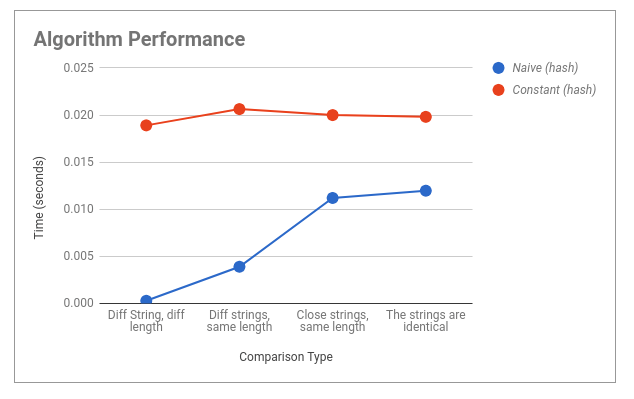
\includegraphics[width=0.8\textwidth]
        {alg_perf.png}
\end{center}



\pagebreak

\printbibliography[heading=bibintoc]

\end{document}
